\newpage
\section{Time Evolution of Closed Quantum Systems}

\subsection{Time-Evolution Operator}
Apply an operator on a state-vector when the system evolves in time. Given the state of a system $\ket{\psi(0)}$ at time $t=0$, the state of the system at time $t$ can be expressed as 
\begin{align*}
    \ket{\psi(t)}=U(t)\ket{\psi(0)}
\end{align*}
where $U(t)$ is called the time-evolution operator. While measurements are probabilistic and irreversible in general, the time evolution of the state-vector is deterministic and reversible. 

Principle 5: The evolution of state-vectors with time is unitary, i.e.
\begin{align*}
    U^{\dagger}U=I
\end{align*}
If $U$ is unitary, and if $\ket{a}$ and $\ket{b}$ are any two state-vectors, then the inner product of $\ket{a'}=U\ket{a}$ and $\ket{b'}=U\ket{b}$ is the same as the inner product of $\ket{a}$ and $\ket{b}$, i.e.
\begin{align*}
    \braket{a'|b'}=\braket{a|U^\dagger U |b}=\braket{a|b}
\end{align*}
\begin{itemize}
    \item If $\ket{a}$ is normalized, so is $U\ket{a}$. 
    \item If $\ket{a}$ and $\ket{b}$ are distinguishable, i.e. $\braket{a|b}=0$, so are $U\ket{a}$ and $U\ket{b}$. That is, information (or distinction) is never lost. 
\end{itemize}

Consider the time-evolution operator $U(\epsilon)$ for infinitesimal $\epsilon$, and seek a differential equation for the evolution of the state-vector. The operator must satisfy
\begin{itemize}
    \item Unitarity\begin{align*}
        U^\dagger (\epsilon)U(\epsilon)=I
    \end{align*}
    \item Continuity\begin{align*}
        U(\epsilon)=U(0)+\frac{\epsilon}{i\hbar}H
    \end{align*}
    where $U(0)=I$ and $-\frac{i}{\hbar}$ is included by convention. 
\end{itemize}

Putting them together, we have\begin{align*}
    \left( I+\frac{\epsilon}{i\hbar}H \right)^\dagger \left( I+\frac{\epsilon}{i\hbar}H \right)=I
\end{align*}
which, in the leading order $O(\epsilon)$, leads to $H^\dagger -H=0$.

Thus, we find that $H$ defined in the continuity condition is Hermitian, $H^\dagger = H$. 

Further, $H$ can be identified as the quantum Hamiltonian. According to the definition, \begin{align*}
    \ket{\psi(t+\epsilon)}=\ket{\psi(t)}+\frac{\epsilon}{i\hbar}H\ket{\psi(t)}
\end{align*}
Taking the limit as $\epsilon\rightarrow 0$,\begin{align*}
    \lim_{\epsilon \rightarrow 0} \frac{\ket{\psi(t+\epsilon)}-\ket{\psi(t)}}{\frac{\epsilon}{i\hbar}}=i\hbar\frac{\partial \ket{\psi(t)}}{\partial t}=H\ket{\psi(t)}
\end{align*}
which is the time-dependent Schroedinger equation. 


\subsection{Manipulating Qubits: Rabi Oscillations}

\subsubsection{Spin in a Magnetic Field}
If we know the Hamiltonian of a system (and its initial state), we can calculate how the state of the system evolves with time. $H$ can be identified with the classical concept of a Hamiltonian, and its eigenvalues with energy.In general, we can derive it from experiment, or borrow it from the classical theory. Sometimes, we can pick one based on symmetry or just experience.

In the case of a single spin, the choice is obvious. All $2\times 2$ Hermitian matrix can be expanded as a linear combination of the identity matrix $I$ and Pauli matrices.
\begin{align*}
    H&=\begin{pmatrix}
        a & b\\c&d
    \end{pmatrix}=H^\dagger=\begin{pmatrix}
        \bar{a} & \bar{c}\\\bar{b}&\bar{d}
    \end{pmatrix}\\
    \therefore\ H&=\begin{pmatrix}
        r_1 & \alpha_i\beta\\ \alpha+i\beta & r_2
    \end{pmatrix}\\
    &=a_1 I +a_2 \sigma_x+a_3 \sigma_y+a_4 \sigma_z
\end{align*}

Spin is a 3-vector, and it must find another 3-vector to make a scalar operator $H$. In the magnetic field, this is the obvious choice, so\begin{align*}
    H\sim -\vec{\sigma}\cdot\vec{B}=-\begin{pmatrix}
        B_z & B_x-iB_y\\ B_x+iB_y&-B_z
    \end{pmatrix}
\end{align*}

In particular, we consider a simple example in which $\vec{B}=B_z\hat{z}$. For convenience, we often write\begin{align*}
    H_0=-\frac{\hbar\omega_0}{2}\sigma_z
\end{align*}
In which we absorb $B_z$ into the frequency $\omega_0$. 
\begin{itemize}
    \item The Hamiltonian has two eigenvalues $\pm \frac{\hbar\omega_0}{2}$, and the corresponding eigenstates are $\ket{0}$ and $\ket{1}$. 
    \item The minus sign is a convention, such that $\ket{0}$ or ``spin up'' is the ground state.
    \item The system can absorb or emit a photon of energy $\hbar \omega_0$, which can be measured experimentally.
\end{itemize}

Since $H_0$ is independent of time, we can solve the time-evolution equation \begin{align*}
    i\hbar\frac{\partial \ket{\psi(t)}}{\partial t}=H_0\ket{\psi(t)}
\end{align*}
by symbolic integration to give 
\begin{align*}
    \ket{\psi(t)}\equiv U_0(t)\ket{\psi(0)}=e^{ -iH_0 t/\hbar }\ket{\psi(0)}
\end{align*}
where $\ket{\psi(0)}$ is the state-vector at $t=0$. 

In practice, we find all the eigenvalues and eigenvectors
\begin{align*}
    H\ket{j}=E_j\ket{j}
\end{align*}
Expand the initial state $\ket{\psi_0}$ with the eigenvector basis
\begin{align*}
    \ket{\psi(t=0)}=\sum_j\ket{j}\braket{j|\psi_0}
\end{align*}
The evolution of the state-vector is 
\begin{align*}
    \ket{\psi(t)}=\sum_j\ket{j}\braket{j|\psi_0}e^{-iE_jt/\hbar}
\end{align*}

The initial state can be written, in the $\sigma_z$ basis (in which $H_0$ is diagonal), as
\begin{align*}
    \ket{\psi(0)}=\cos\frac{\theta}{2}\ket{0}+\sin\frac{\theta}{2}\ket{1}
\end{align*}
The time-evolution operator, in the same basis, is
\begin{align*}
    U_0(t)&=e^{(-iH_0t/\hbar)\sigma_z}=e^{i(\omega_0 t/2)\sigma_z}=\begin{pmatrix}
        e^{i\omega_0 t/2} & 0\\ 0& e^{-i\omega_0 t/2}
    \end{pmatrix}\\
    &=e^{i\omega_0 t/2}\ket{0}\bra{0}+e^{-i\omega_0 t/2}\ket{1}\bra{1}
\end{align*}
Therefore, the state-vector at time $t$ is 
\begin{align*}
    \ket{\psi(t)}=e^{i\omega_0 t/2}\cos\frac{\theta}{2}\ket{0}+e^{-i\omega_0 t/2}\sin\frac{\theta}{2}\ket{1}
\end{align*}
Owing to the arbitrary overall phase, we can write
\begin{align*}
    \ket{\psi(t)}=\cos\frac{\theta}{2}\ket{0}+e^{-i\omega_0 t}\sin\frac{\theta}{2}\ket{1}
\end{align*}
The state-vector on the Bloch sphere precesses about $\hat{z}$-axis with an angular frequency $\omega_0$.

It is interesting to note that if we absorb the phase into the basis
\begin{align*}
    \ket{0}\rightarrow\ket{0'}\equiv e^{i\omega_0 t/2}\ket{0},\ \ket{1}\rightarrow\ket{1'}\equiv e^{-i\omega_0 t/2}\ket{1}
\end{align*}
the state “remains” unchanged as
\begin{align*}
    \ket{\psi(t)}=\cos\frac{\theta}{2}\ket{0'}+\sin\frac{\theta}{2}\ket{1'}
\end{align*}
In other words, in the so-called \hl{rotating reference frame}, the state vector remains unchanged, i.e., the effective Hamiltonian in the rotating frame is $H'=0$. (将操作旋转到了坐标轴)

\subsubsection{Interaction Picture}
In this so-called the interaction picture, the basis is defined, in general, by
\begin{align*}
    \ket{n'}=U_0(t)\ket{n}
\end{align*}
so we redefine the wave function and the observables $\hat{O}$
\begin{align*}
    \ket{\psi_I (t)}=U_0(t)^\dagger \ket{\psi(t)},\ \hat{O}_I=U_0(t)^\dagger \hat{O}U_0(t)
\end{align*}

One can check that the probability density and expectation values remain unchanged
\begin{align*}
    \braket{n|\psi_I}=\braket{n'|\psi},\ \braket{\psi_I|\hat{O}_I|\psi_I}=\braket{\psi|\hat{O}|\psi}
\end{align*}
In this frame the new wave function is dictated by an interaction-picture Hamiltonian
\begin{align*}
    i\hbar\frac{\partial}{\partial t}\ket{\psi_I}&=H_I(t)\ket{\psi_I}\\
    &=\left[ U_0(t)^\dagger H(t)U_0(t)-i\hbar U_0(t)^\dagger \left( \frac{\partial}{\partial t}U_0(t) \right) \right]\ket{\psi_I}
\end{align*}

\subsubsection{Manipulating a Spin (Qubit)}
A constant $\vec{B}=B_z\hat{z}$ does not transform a state, e.g., from $\ket{0}$ to an arbitrary linear superposition of $\ket{0}$ and $\ket{1}$. 

This can be done by applying, in addition to a constant $B_z$ , a magnetic field $\vec{B}_1(t)$ rotating in the $x$ -$y$ plane with angular frequency $\omega$:
\begin{align*}
    \vec{B}_1(t)=B_1(\cos\omega t \hat{x}-\sin\omega t\hat{y})
\end{align*}
such that the Hamiltonian becomes
\begin{align*}
    H(t)=-\frac{\hbar\omega_0}{2}\sigma_z-\frac{\hbar\omega_1}{2}(\sigma_x\cos\omega t-\sigma_y\sin\omega t)
\end{align*}

For microwave controls, we can use the microwave frequency $\omega$ in the free rotation $U_0(t)=e^{i(\omega t/2)\sigma_z}$. In the interacting picture, therefore, one can show that
\begin{align*}
    U_0^\dagger \sigma_z U_0&=\begin{pmatrix}
        e^{-i\omega t/2} & 0\\0& e^{i\omega t/2}
    \end{pmatrix}\hspace*{-2pt} \begin{pmatrix}
        1 & 0 \\ 0 &-1
    \end{pmatrix}\hspace*{-2pt} \begin{pmatrix}
        e^{i\omega t/2} & 0\\0& e^{-i\omega t/2}
    \end{pmatrix}\\
    &=\begin{pmatrix}
        1 & 0 \\ 0 & -1 
    \end{pmatrix}=\sigma_z\\
    U_0^\dagger \sigma_x U_0&=\begin{pmatrix}
        0 & e^{-i\omega t}\\e^{i\omega t}&0
    \end{pmatrix}\\
    U_0^\dagger \sigma_y U_0&=\begin{pmatrix}
        0 & -ie^{-i\omega t}\\ie^{i\omega t}&0
    \end{pmatrix}
\end{align*}
Therefore, we have, in the rotating frame,
\begin{align*}
    H_I(t)&=\left[ U_0(t)^\dagger H(t) U_0(t)-i\hbar U_0(t)^\dagger\left( \frac{\partial}{\partial t}U_0(t) \right) \right]\\
    &=-\frac{\hbar(\omega_0-\omega)}{2}\sigma_z-\frac{\hbar\omega_1}{2}\sigma_x
\end{align*}
\begin{figure}[H]
    \centering
    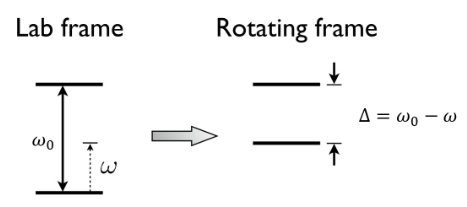
\includegraphics[width=0.309\textwidth]{QI5/The lab frame and the rotating frame}
    \caption{The lab frame and the rotating frame}
\end{figure}


If at time $t=0$ the spin is in the state $\ket{0}$, its probability in state $\ket{1}$ at time $t$ can be calculated to be 
\begin{align*}
    |\braket{1|\psi(t)}|^2=|\braket{1|\psi_I(t)}|^2=\left( \frac{\omega_1}{\Omega} \right)\sin^2\frac{\Omega t}{2}
\end{align*}
where $\Omega=\sqrt{(\omega-\omega_0)^2+\omega_1^2}$.

This is the phenomenon of \hl{Rabi oscillations}, which is the basic process to manipulate qubits in quantum computing. These oscillations are obtained by exposing qubits to periodic electromagnetic fields during suitably adjusted time intervals.

\subsection{Recap of the Quantum Theory in General Physics}
The state of a quantum particle is represented by a wave function $\psi(\vec{r},\ t)$. 

The time evolution of the state $\psi(\vec{r},\ t)$ of a non-relativistic particle is governed by the Schroedinger equation
\begin{align*}
    i\hbar\frac{\partial \psi}{\partial t}=H\psi
\end{align*}
where the Hamiltonian fo conserved forces is 
\begin{align*}
    H=-\frac{\hbar^2}{2m}\nabla^2 +U(\vec{r},\ t)
\end{align*}
where $H$ is independent of time, the wave function can be separated to be $\psi(\vec{r},\ t)=\phi(\vec{r})e^{-iEt/\hbar}$, which satisfies
\begin{align*}
    H\phi=E\phi
\end{align*}

The probability of finding the particle somewhere at a particular time is proportional to $|\psi(\vec{r},\ t)|^2$. A particle in a potential trap is only allowed to have discrete energy levels. The particle can absorb light and gain energy or emit light and lose energy. Only photons whose energies (or colors) match the ``jump'' in energy levels can be emitted or absorbed. 

We have encountered the following wave functions to describe the state of a particle. 
\begin{itemize}
    \item A 1D particle localized at $x = x_0$ has a wave function $\psi(x ) = \delta(x - x_0)$, where $\delta(x)$ is the Dirac delta function. This is a real-space eigenstate. 
    \item A particle moving along the $x$ direction with momentum $\hbar k$ has a wave function $\psi(x ) = e^{ikx}$ . This is a momentum-space eigenstate. 
    \item The electron in the ground state of a hydrogen atom has a wave function $\psi(\vec{r})=e^{-r/a_B}$, where $a_B$ is the Bohr radius. This is neither a real-space eigenstate nor a momentum-space eigenstate. 
\end{itemize}

\subsubsection{Heisenberg vs Schroedinger}
\begin{enumerate}
    \item Heisenberg invented one with vectors, linear operators and their algebra. 
    \item Schroedinger thought in terms of wave functions and wave equations. 
\end{enumerate}

The two approaches can be united: wave functions form a vector space, while derivatives are operators.

\subsubsection{What are Wave Functions, Really?}
Suppose we have an orthogonal basis labelled by $\ket{a,b,c,\dots}$, where $a,b,c,\dots$ are eigenvalues of some complete set of commuting observables $A, B, C$. An arbitrary state vector can be expanda as
\begin{align*}
    \ket{\Psi}=\sum_{a,b,c,\dots} \psi(a,b,c,\dots)\ket{a,b,c,\dots}
\end{align*}
The set of coefficients $\psi(a,b,c,\dots)=\braket{a,b,c,\dots|\Psi}$ is called the \textbf{wave function} of the system in the basis defined by the observables $A,B,C,\dots$. 

We can only choose labels that are not conflicting. In the quantum theory, this means observables $A$ and $B$ commute, i.e., $[A,B]\equiv AB-BA =0$. As a consequence, 
\begin{align*}
    AB\ket{a,b,c,\dots}=BA\ket{a,b,c,\dots}=ab\ket{a,b,c,\dots}
\end{align*}

The probability for the commuting observables to have values $a,b,c,\dots$ is 
\begin{align*}
    P(a,b,c,\dots)=\psi^{*}(a,b,c,\dots)\psi(a,b,c,\dots)
\end{align*}
with 
\begin{align*}
    \sum_{a,b,c,\dots}\psi^{*}(a,b,c,\dots)\psi(a,b,c,\dots)=1
\end{align*}

\subsection{Continuous Functions as Vectors}
It can be shown that complex functions form a complex vector space, or a \textbf{Hilbert space}. 

But to translate the principles of quantum mechanics bewteen vector-based ideas (Heisenberg) to function-oriented ideas (Schroedinger), we need the following recognitions
\begin{enumerate}
    \item Integral repalce sum.
    \item Dirac delta function repalce Kronecker delta.
    \item Probability density repalce probability. 
\end{enumerate}

\subsubsection{Integral Replace Sum}
Consider a ket-vector $\ket{\psi}=\sum\limits_i \alpha_i\ket{i}$. The basis $\ket{i}$ gets translated to a continuous basis $\ket{x_i}$, which describes a particle at $x_i$. The analogy to the state vector is (notice $\sum\limits_i \rightarrow \int \mathrm{d}x$)
\begin{align*}
    \ket{\psi}=\int \mathrm{d}x_i\psi(x_i) \ket{x_i}
\end{align*}

Therefore, the wave function, as the coefficient $\alpha_i=\braket{i|\psi}$, is 
\begin{align*}
    \psi(x)=\braket{x|\psi}
\end{align*}

Strictly speaking, $\psi(x)$ isn't a state, which we call $\ket{\psi}$. 

\subsubsection{Dirac Delta Function Replace Kronecker Delta}
To have teh algebra self-consistent, we have
\begin{align*}
    \psi(x)=\braket{x|\psi}=\int \mathrm{d}x_i\psi(x_i)\braket{x|x_i}
\end{align*}

In the vector-based description, $\braket{j|i}=\delta_{ij}$. It is natural ti identify $\braket{x|x_i}=\delta(x-x_i)$, the Dirac delta function, which satisfies
\begin{align*}
    \int_{-\infty}^{\infty}\mathrm{d}x\delta(x-x')&=1\\
    \int_{-\infty}^{\infty}f(x')\delta(x-x')\ \mathrm{d}x'&=f(x)
\end{align*}

Thus, we can interpret $\braket{x_i|x_j}=\delta(x_i-x_j)$ as the orthogonality of the basis vectors. 

\subsubsection{Probability Density Replace Probability}
The normalization of the ket-state is
\begin{align*}
    \braket{\psi|\psi}=\sum_i\braket{\psi|i}\braket{i|\psi}=\sum_i\alpha_i^\dagger\alpha_i=1
\end{align*}
where we have inserted the completeness condition\\ $\sum\limits_i\ket{i}\bra{i}=1$. 

The continuum version would be 
\begin{align*}
    \braket{\psi|\psi}=\int \mathrm{d}x\braket{\psi|x}\braket{x|\psi}=\int \mathrm{d}x\psi^*(x)\psi(x)=1
\end{align*}

We can identify the completeness condition as, symbolically
\begin{align*}
    \int\mathrm{d}x\ket{x}\bra{x}=1
\end{align*}
The product $\psi^*(x)\psi(x)$ is known as the \textbf{probability density}. 